\documentclass[11pt]{article}
\usepackage{graphicx}
\usepackage{float}

\begin{document}
	\title{Ticket Salad Coding Standards}
	\date{}
	\maketitle
	\tableofcontents
	\newpage
	
	\section{Introduction}
	\subsection{Purpose}
	The goal of these guidelines is to create uniform coding habits among software personnel in the
	engineering department so that reading, checking, and maintaining code written by different persons
	becomes easier. The intent of these standards is to define a natural style and consistency, yet leave
	to the authors of the engineering department source code, the freedom to practice their craft without
	unnecessary burden
	\subsection{Scope}
	This document describes general software coding standards for code written in HTML, SCSS, Javascript and Mongo.
	\subsection{Terms used in this document}
	\textbf{Element: }Element refers to a structure or some data that is used in an HTML file, e.g: <h1>
	\section{HTML Guidelines}
	\subsection{Naming requirements}
	Naming conventions form a major part of coding standards as it makes code more readable by other developers thus increasing the scalability of the software.
	\subsubsection{File names}
	HTMl files names are short, preferably one word names based directly on the html pages direct purpose.
	\textbf{e.g} A login page will be named 'LogIn.html'. 
	\subsubsection{Class names and ID names}
	Classes are applied to many different elements in the HTML, therefore they are not very unique and describe a general purpose or layout preference for that element.
	ID attributes are uniquely applied to different elements. Therefore they are unique and describe what is unique about that element. 
	\textbf{e.g} A class that is used for icons on the webpage will have a class: 'icon. A element that serves a unique role such as a login button will be have id: 'login'
	\subsection{Formatting requirements}
	The layout of code plays a large part in the ability for someone else to read the code as it allows for the readers ability to "flow" through the code to be improved because there is a logical layout.
	\begin{itemize}
		\item Sub-elements are indented by one space to the right compared to their parent element.
		\item White lines are used to break up large amounts of code into more understandable subsections of the HTML page.
		\item There is no unnecessary whitespace in the HTML document.
		\item Every element is on a new line.
	\end{itemize}
	\subsection{In-code comment requirements}
	Comments are crucial to the ability to understand code because if another developer cannot identify the purpose of the specific section of code they can address the comments.
	
	In HTML comments are not as necessary compared to other languages, however is required in some cases. However over commenting a file is avoided.
	\begin{itemize}
		\item Comments are not made on elements that can be identified using their classes and ID's
		\item Comments are made when the page calls any javascript functions, this comment will describe the function that is being called.
		\item Comments are made if the purpose of an element is not visible.
		\item Comments are made to describe the purpose of a large segment of code.
	\end{itemize}
	\section{CSS Guidelines}
	\subsection{Naming requirements}
	Naming conventions form a major part of coding standards as it makes code more readable by other developers thus increasing the scalability of the software.
	\subsubsection{File names}
	CSS files are named according to HTML file they relate to. \textbf{e.g} A CSS file used to style the login page will be called 'login.css'
	\subsubsection{Class names and ID names}
	Class and id names relate directly to the class and id names defined in the html.
	\subsection{Formatting requirements}
	The layout of code plays a large part in the ability for someone else to read the code as it allows for the readers ability to "flow" through the code to be improved because there is a logical layout.
	\begin{itemize}
		\item White lines are used to break up large amounts of code into more understandable subsections of the css page.
		\item There is no unnecessary whitespace in the CSS document.
		\item Every statement is on a new line.
	\end{itemize}
	\subsection{In-code comment requirements}
	Comments are crucial to the ability to understand code because if another developer cannot identify the purpose of the specific section of code they can address the comments.
	
	In CSS, comments are not used as the class names and id names are descriptive therefore comments are not needed.
	
	\section{Javascript Guidelines}
	\subsection{Naming requirements}
	Naming conventions form a major part of coding standards as it makes code more readable by other developers thus increasing the scalability of the software.
	\subsubsection{File names}
	Javascript files are named according to the HTML page the script will be applied to followed by '.controller'.\textbf{e.g} The javascript file for the login page will be called 'login.controller.js'
	
	Javascript files that are applied to many pages and serve a more general purpose, are named according to their purpose.
	\subsubsection{Variable names}
	Variable names form a crucial part of coding standards in javascript as all variables serve a specific purpose.
	\begin{itemize}
		\item Variable names describe what data will be stored by a variable\textbf{e.g} A variable used to store a users id will be named id.
		\item Variable names are short and descriptive
		\item Variable names use a camelCasing style.
		\item 'Magic numbers' are not used and instead are assigned to predefined constants.
		\item Predefined constants are uppercase.
		\item Variable names are consistent throughout all the Javascript files if they store the same data. 
	\end{itemize}
	\subsubsection{Function names}
	Function names are used to call that function's code in other parts of the document and other files. If function names are random and non-descriptive the purpose of that function will not be easily identifiable.
	\begin{itemize}
		\item Function names are short and descriptive. \textbf{e.g} A function that is used to calculate a users credits will be called 'calculateCredits()'.
		\item Function names follow the camelCasing style.
	\end{itemize}
	\subsection{Formatting requirements}
	The layout of code plays a large part in the ability for someone else to read the code as it allows for the readers ability to "flow" through the code to be improved because there is a logical layout.
	\begin{itemize}
		\item Each statement of code is on a new line.
		\item White lines are used to break up large amounts of code into more understandable subsections of the javascript page.
		\item There is no unnecessary whitespace in the javascript document.
		\item Every curly brace is on a new line
		\item Code blocks are indented by a tab to the left compared to the parent structure.
	\end{itemize}
	\subsection{In-code comment requirements}
	Comments are crucial to the ability to understand code because if another developer cannot identify the purpose of the specific section of code they can address the comments.
	
	In javascript comments are essential as not all javascript code effectively describes the purpose of that code.
	\begin{itemize}
		\item Comments are not made on variables that have a descriptive name
		\item Comments are made on all functions except very simple ones, describing the purpose of the function.
		\item Comments are made if the purpose of an block of code is not visible.
		\item Comments are made to describe the purpose of a large segment of code.
	\end{itemize}
	\subsection{File Headers}
	File headers are included in all the javascript files describing the following aspects.
	\begin{itemize}
		\item File name
		\item Version
		\item Organization name
		\item Project name                                                                                                                                                                                                                                                                                                                                                                                                                                                                                                                                                                                                                                                                                                                                                                                                                                                                                                                                                                                                                                                                                                                                                                                                                                                                                                                                                                                                                                                                                                                                                                                                                                                                                                                                                                                                                                                                                                                                                                                                                                                                                                                                                                                                                                                                                                                                                                                                                                                                         
		\item Functional description
	\end{itemize}
	
	\section{Rules and requirement}
	\subsection{Review Method}
	Upon creation of the Coding Standards the entire development team reviews the coding standards and present them to the stakeholders. If there is a concern it is raised and there is a discussion and if everyone agrees on the change a change is made.
	
	All code changes before a commit to the development branch are reviewed by code shepards Brandon Teixeira and Jarryd Baillie. The shepards will sit down with the changes and the Coding Standards document in front of them. The shepard will then ensure that all the coding requirements for that language is followed.
	
	\subsection{Application of coding standards}
	All files will have to comply to the coding standards including the testing files and structure.
	
	\newpage
	
	\section{GIT file structure}
	\begin{itemize}
		\item All .js files are stored in the controllers folder.
		\item All .css files are stored in the styles folder.
		\item All .html files are stored in the templates folder.
		\item All documentation is stored in the documentation folder.
	\end{itemize}
	\begin{figure}[H]
	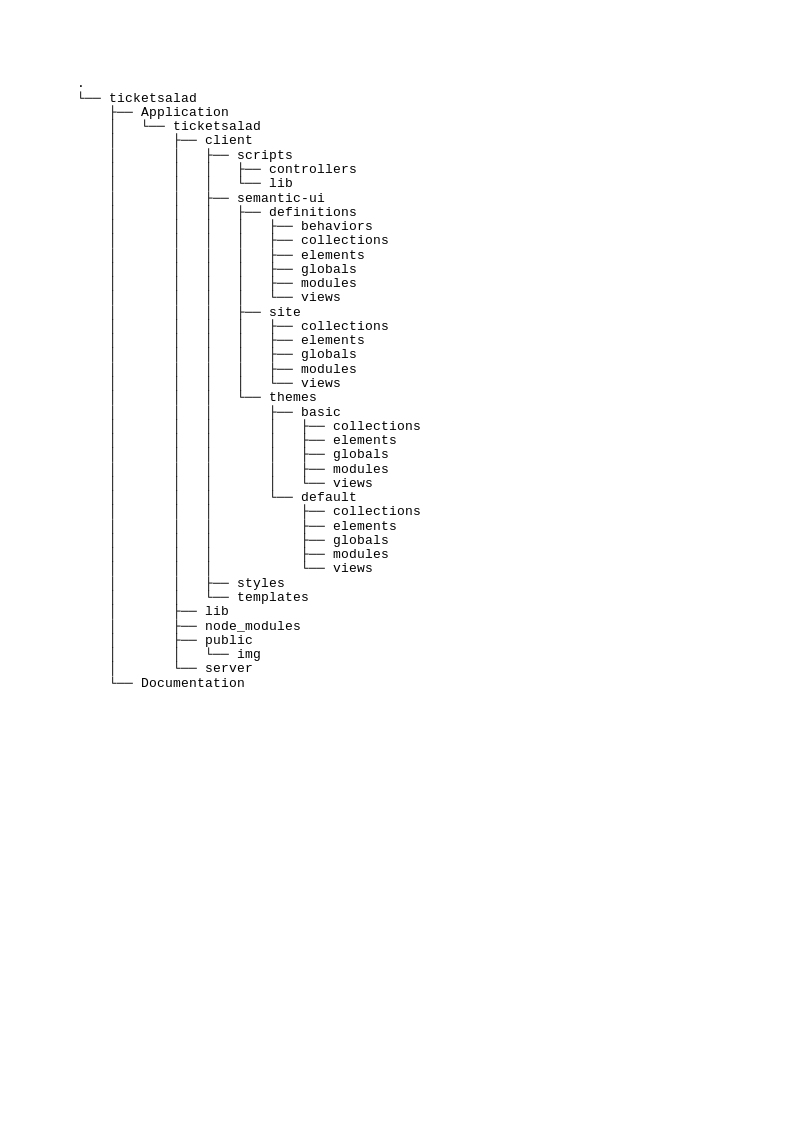
\includegraphics[scale=0.5]{tree}
	\end{figure}
	

	
	
	
\end{document}